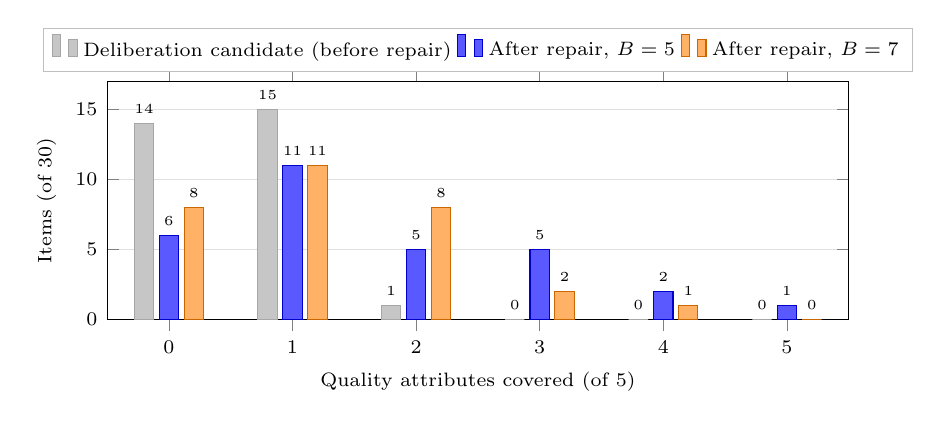
\begin{tikzpicture}
\begin{axis}[
  width=11cm, height=4.6cm, ybar, bar width=7pt, ymin=0, ymax=17,
  xlabel={Quality attributes covered (of 5)}, ylabel={Items (of 30)},
  xtick={0,1,2,3,4,5}, font=\scriptsize, ymajorgrids, grid style={gray!25},
  legend style={font=\scriptsize, at={(0.5,1.04)}, anchor=south, legend columns=3, draw=gray!50},
  nodes near coords, every node near coord/.append style={font=\tiny},
]
\addplot[fill=gray!45, draw=gray!70] coordinates {(0,14) (1,15) (2,1) (3,0) (4,0) (5,0)};
\addplot[fill=blue!65, draw=blue!80!black] coordinates {(0,6) (1,11) (2,5) (3,5) (4,2) (5,1)};
\addplot[fill=orange!60, draw=orange!80!black] coordinates {(0,8) (1,11) (2,8) (3,2) (4,1) (5,0)};
\legend{{Deliberation candidate (before repair)},{After repair, $B=5$},{After repair, $B=7$}}
\end{axis}
\end{tikzpicture}
